\documentclass[a4paper, 12pt]{article}
\usepackage[margin=0.8in]{geometry}
\usepackage{tikz}
\usepackage{scrextend}
\usetikzlibrary{automata,positioning}
\usepackage{graphicx}
\usepackage{listings}
\usepackage{color}

\definecolor{comments}{rgb}{0,0.5,0.5}
\definecolor{typeWord}{rgb}{0.5,0,1}
\definecolor{number}{rgb}{1,0.5,0}
\definecolor{string}{rgb}{0.5,0.5,0.5}

\lstset{frame=tb,
  language=Java,
  aboveskip=3mm,
  belowskip=3mm,
  showstringspaces=false,
  columns=flexible,
  basicstyle={\small\ttfamily},
  numbers=none,
  numberstyle=\color{number},
  commentstyle=\color{comments},
  stringstyle=\color{string},
  keywordstyle=\color{typeWord},
  breaklines=true,
  breakatwhitespace=true,
  tabsize=4
}

\title{Scotland Yard}
\author{Julian Loscombe and Ben Milne}

\begin{document}
\maketitle
\section{Project Schematic}
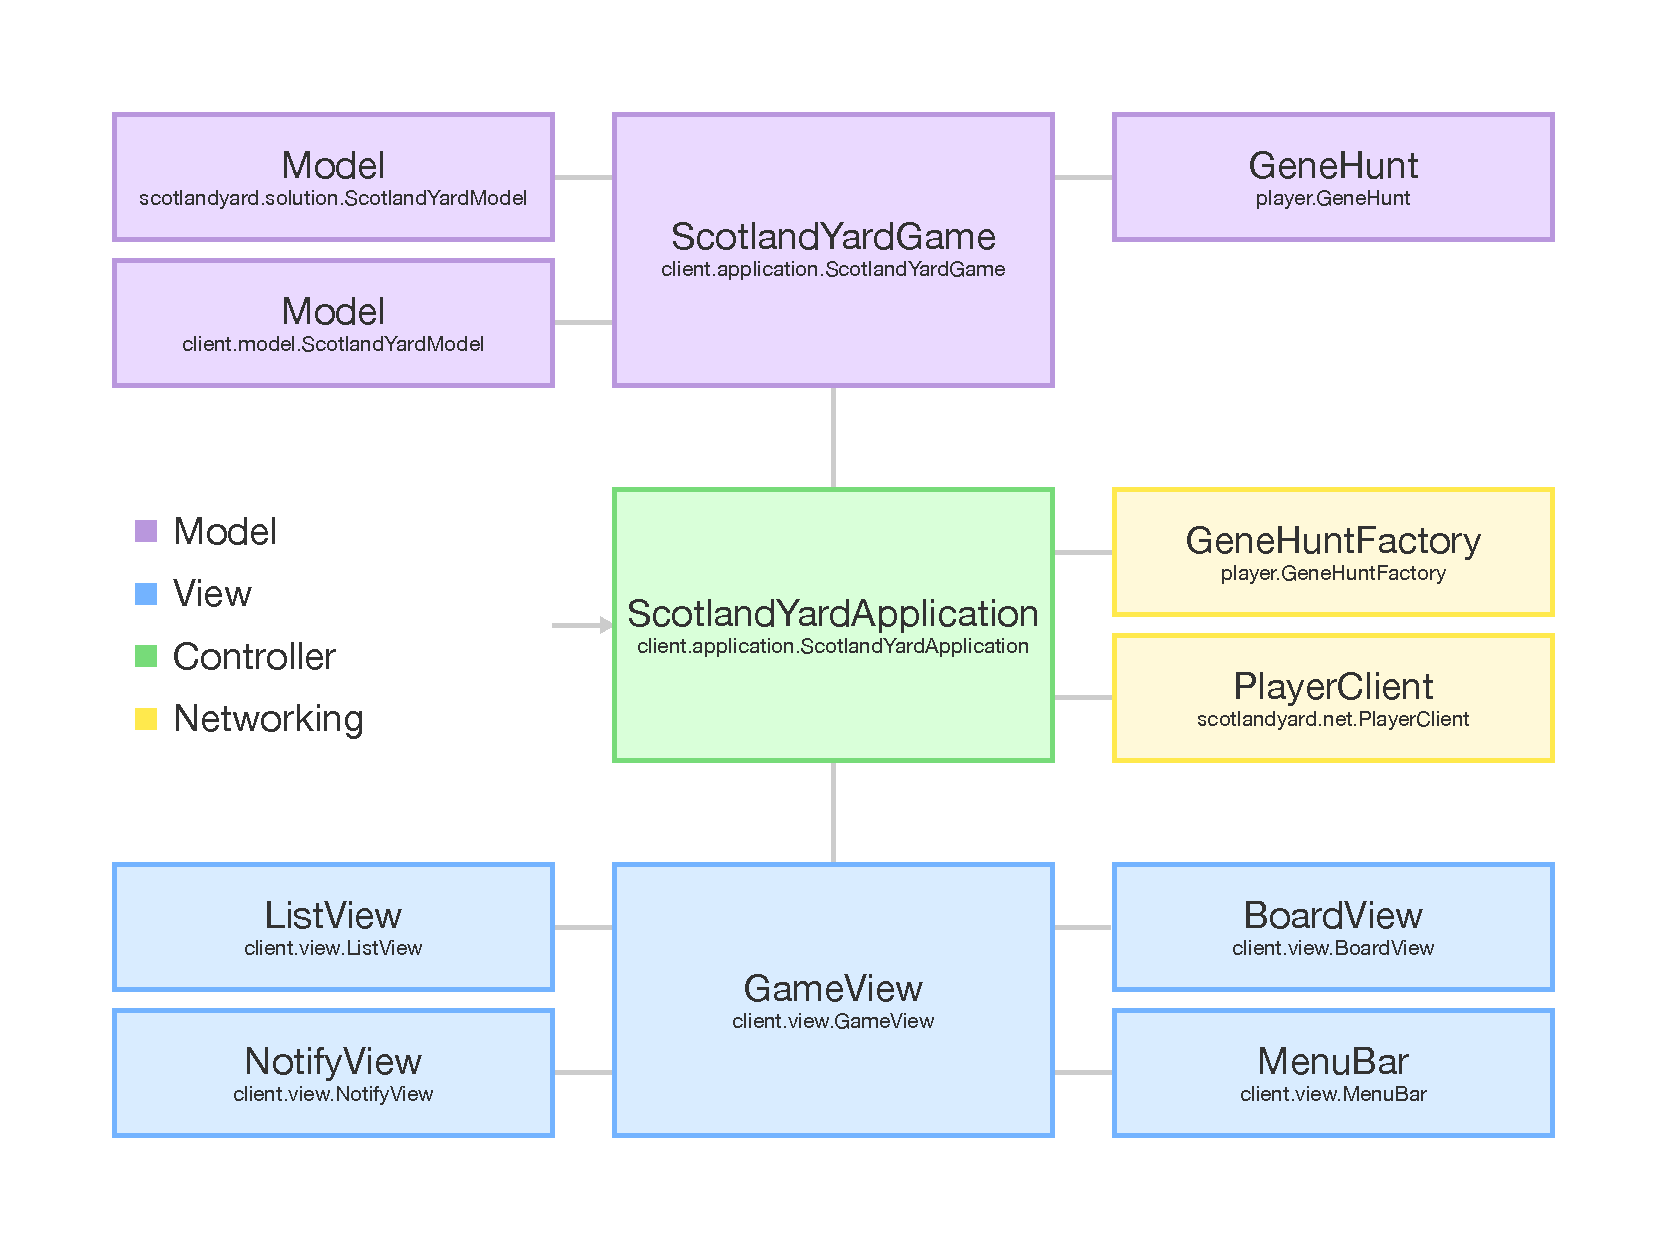
\includegraphics[width = 17cm]{mvp_schematic}\\
As our project grew it became important to organise our code. To achieve this we came up with the above project structure. You can clearly see the separation of the model and the views.
\section{Animations}
In the first part of the project we did not have sufficient time to add animations to the game. We feel these are important as they guide your attention and allow you to keep track of what is happening more easily. In order to easily implement our animations in this part we created a class called AnimatablePanel which is documented separately.
\section{Benefits of our GUI}
We decided early on to use our own GUI, this is because we feel our GUI has four main advantages over the one provided. Our GUI:
\begin{enumerate}
	\item Automatically make a random move when the time to take a move runs out. Therefore the game will not quit if you take too long.
	\item Allows panning and zooming which especially useful for low resolution screens. The provided GUI does not resize and hence on some screens a potion of the board is cut off and unreachable.
	\item Shows the suggested routes generated by the AI and all the valid moves you can take.
	\item Shows the time remaining for you to make a move clearly, we found the timer on the provided guy was often off screen and impossible to see.
\end{enumerate}
\section{Disadvantages of our GUI}
Although we are generally very pleased with our GUI, we have found some limitations of it:
\begin{enumerate}
	\item It is difficult to see what moves Mr X has previously made as we have used a chat view to communicate game events. In hindsight this is not the best method and the provided GUI is much better at this. We decided to use this method before we knew the limitations of the networking, hoping to enable client to client chat.
	\item It is very difficult to see what tickets other players are holding. Again we hoped to mitigate this issue using the chat.
\end{enumerate}
\section{The horrible bug with the networking}
When connecting our GUI to the networking part of the project, we encountered a difficult to trace bug, as you may remember. The problem was that the PlayerClient class calls model.start() in the run() method, but we also called model.start() on another thread as we did not know that it had already been done. This meant that the game was effectively started twice on two Threads causing havoc with the updating of our GUI. To solve this problem we changed our code so only the PlayerClient called the model.start() method. It would have been helpful to either add the synchronised tag to the model.start() method so in debugging it would be easier to spot that it was being run twice or an even simpler solution would be to add some documentation about the PlayerClient class.
\section{The second horrible bug with the networking}
We would often find when running our AI that the server would end the game before we had a chance to make our first move (i.e before 15 seconds after entering the notify function). We performed the below test to ensure it was not an issue with our GUI but with the server itself.
\\
\begin{lstlisting}
public class RandomPlayer implements Player {

	...
	
	@Override
	public Move notify(int location, Set<Move> moves) {
		try {
			Thread.sleep(14000);
		} catch (Exception e) {}
		
		...
		
		return move;
	}
	
	...
	
}
\end{lstlisting}
\hfill \break
When we run the above code which is in the RandomPlayer class supplied with the basis of the project, the game is over before Mr X makes his first move. As this is in the RandomPlayer class, it is used by the supplied GUI and hence it could not be a problem with our GUI - this leads us to believe it is a problem with the server. If we reduce the time to 10 seconds, the game is not over and Mr X is able to make his move. Even though the Thread.sleep() method is not accurate, from our testing it only waits less than 5 milliseconds longer than the specified time which doesn't make up for the other 995 milliseconds - so the inaccuracy of the Thread.sleep() method is not to blame.
\\
\\
This means we do not get the full 15 seconds to compute the move for Mr X on the first round of the game and have had to implement a kind of messy work around for it. On subsequent rounds of the game, this problem doesn't persist leading us to the conclusion that it is caused by a blocking operation when the game starts causing the notify method's call to be delayed.
\\
\\
The most annoying thing with this bug is that it is intermittent and we believe this to be because Java is not a real-time programming language and is therefore highly dependent on OS scheduling, so this will contribute to the time not being consistent and hence this is what we think is the real cause of the issue and the only way to get around it in the standard edition of Java is to use a ScheduledExecutorService or a custom Timer.
We first spent a lot of time trying to figure out where our AI was going wrong before we realised it was actually a problem with the server/Java creating a bit of frustration.
\section{Transitional Issues}
The update to the project files part-way through the project (when we switched to the new scotlandyard package) caused a significant lag ($\sim$10s) when starting a new game. We tracked this down to the Page Rank algorithm, specifically the iterate() method which is called 100 times at the beginning of a game. In order to see clearly where the problem was we used the System.nanoTime() method to find the time each line of the method took.\\
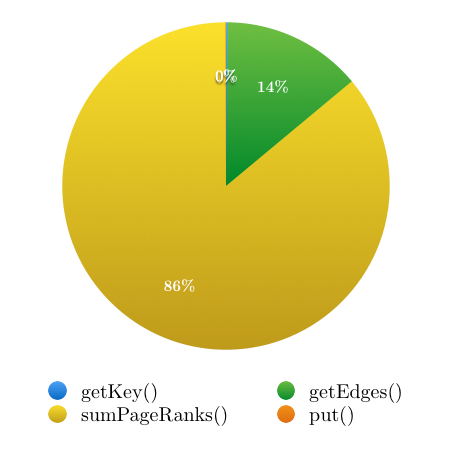
\includegraphics[width = 8cm]{iterate}
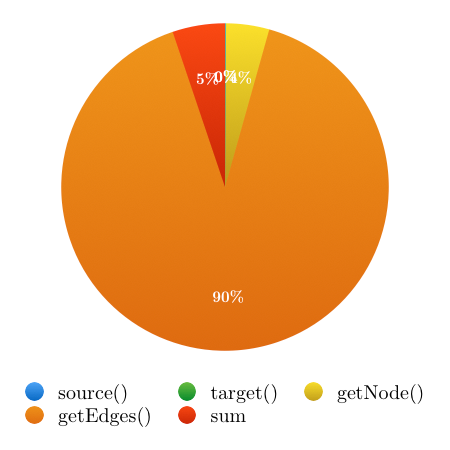
\includegraphics[width = 8cm]{sumPageRanks}\\
\\
Clearly then, the issue is with the getEdges() method in the Graph file. We believe this is because of the change from using Lists to Sets. The cost of iterating over a Set, it seems, is far greater than doing the same for a List as illustrated at http://javacodegeeks.com/2010/08/java-best-practices-vector-arraylist.html.\\
\\
To fix this we created a map on itilialisation which maps a node number to its edges. This means we only need to iterate over the Set once and the result is a significant speed increase.\\
\centerline{
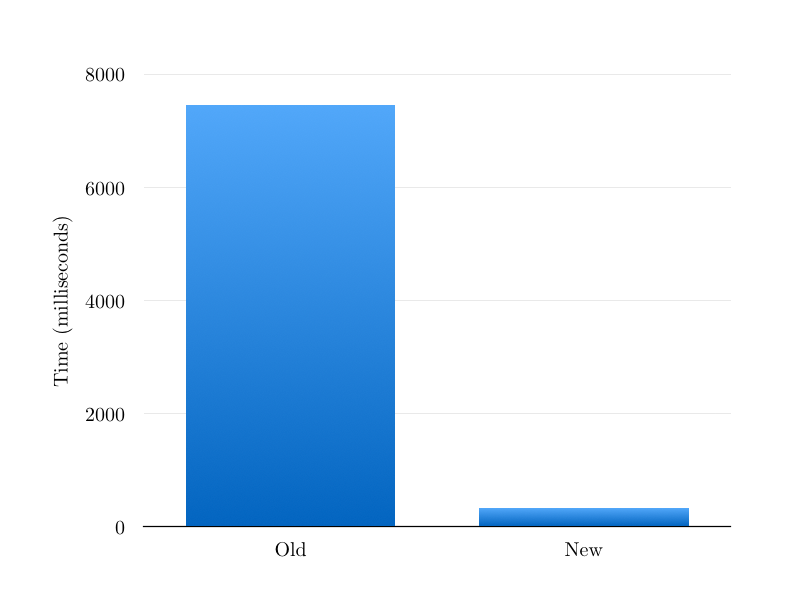
\includegraphics[width = 14cm]{comparison}\\
}
\section{Documentation}
We have fully commented our code to the JavaDoc specifications and have generated the html, you can find it in the docs/Documentation/JavaDocs folder.
\end{document}